\subsection{Tilpasning af filtre}
\label{TilpasningAfFilter}
%
De efterfølgende tabeller lister de beregnede og brugte komponentværdier, afhængigt af hvilket filter de tilhører og hvor stor afvigelsen er. Under hver tabel fremgår det tilhørende, færdige, filter.
%
\begin{equation}
	Afvigelse (\%) = \frac{brugt-beregnet}{beregnet}*100\%
\end{equation}
%
\begin{table}[H]
\centering
\begin{tabular}{|c|r|r|r|}
\hline
\multicolumn{1}{|l|}{Komponenter} & \multicolumn{1}{l|}{Beregnet} & \multicolumn{1}{l|}{Brugt} & \multicolumn{1}{l|}{Afvigelse [$\%$]}\\ \hline
$R_i$ & 10k$\Omega$ & 10k$\Omega$ & 0\\ \hline
$R_F$ & 13.521k$\Omega$ & 13.7k$\Omega$ & 1.3239 \\ \hline
$R_1$ & 127.826k$\Omega$ & 127k$\Omega$ & 0.6462\\ \hline
$R_2$ & 115.598k$\Omega$ & 115k$\Omega$ & 0.5173 \\ \hline
$R_3$ & 104.541k$\Omega$ & 105k$\Omega$ & 0.4391 \\ \hline
$C_1$ & 20.473nF & 22nF & 7.4586 \\ \hline
$C_2$ & 8.604nF & 6.8nF & -20.967 \\ \hline
$C_3$ & 3.62nF & 3.5nF & -3.3149 \\ \hline
\end{tabular}
\caption{Komponentværdier for de filtre der forstærker $\pm$2.62dB.}
\label{tab:TilpasningAfFiltre2.62}
\end{table}
%
\begin{figure}[H]
	\centering
	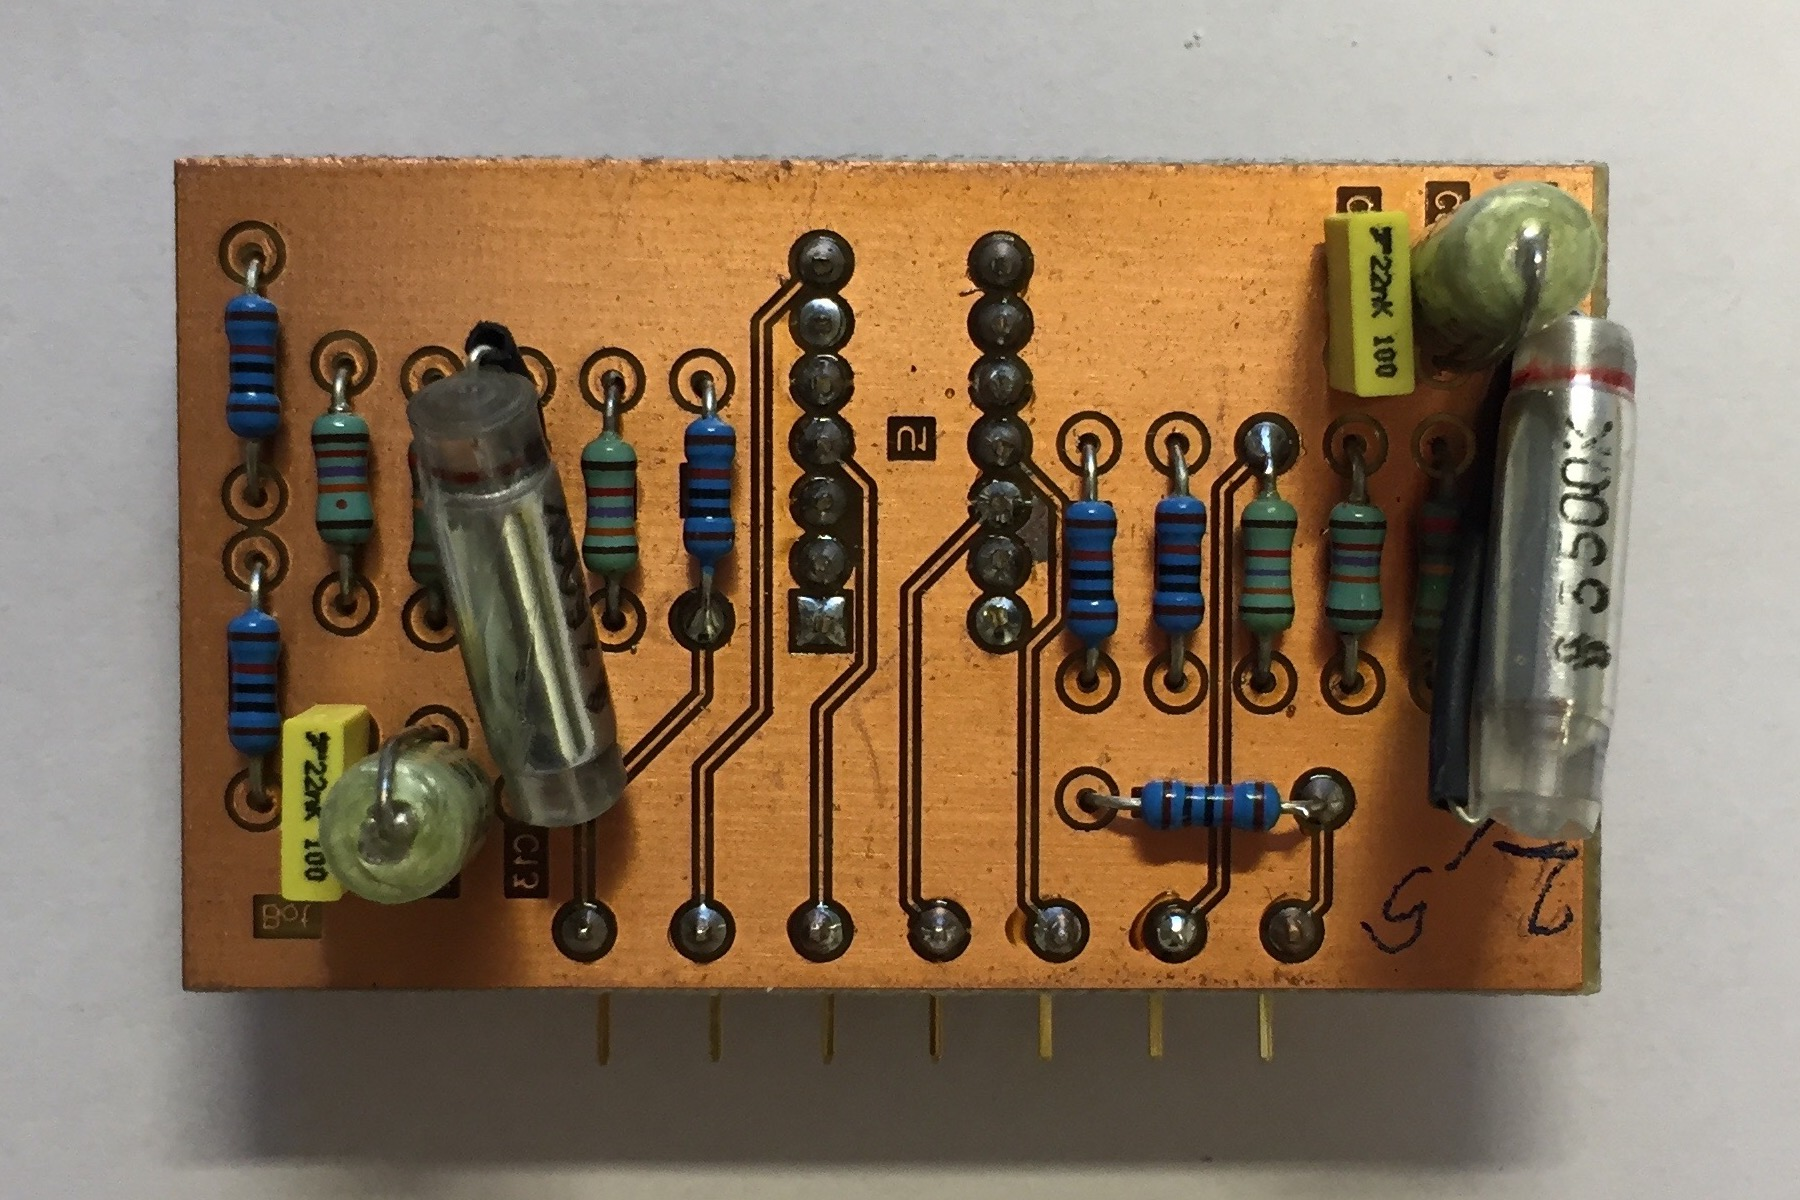
\includegraphics[resolution=300,width=\textwidth/2]{ProductShots/Filter2_5Front}
	\caption{Færdigt filter for $\pm$2.62dB}
	\label{fig:Filter2_5Front}
\end{figure}
\noindent
%
%
\begin{table}[H]
\centering
\begin{tabular}{|c|r|r|r|}
\hline
\multicolumn{1}{|l|}{Komponenter} & \multicolumn{1}{l|}{Beregnet} & \multicolumn{1}{l|}{Brugt} & \multicolumn{1}{l|}{Afvigelse [$\%$]}\\ \hline
$R_i$ & 10k$\Omega$ & 10k$\Omega$ & 0\\ \hline
$R_F$ & 18.281k$\Omega$ & 18.7k$\Omega$ & 2.292 \\ \hline
$R_1$ & 82.074k$\Omega$ & 82.5k$\Omega$ & 0.519 \\ \hline
$R_2$ & 67.123k$\Omega$ & 66.5k$\Omega$ & 0.9281 \\ \hline
$R_3$ & 54.896k$\Omega$ & 54.9k$\Omega$ & 0.0073 \\ \hline
$C_1$ & 28.835nF & 33nF & 14.4443 \\ \hline
$C_2$ & 13.408nF & 15nF & 11.8735 \\ \hline
$C_3$ & 6.235nF & 6.8nF & 9.0617 \\ \hline
\end{tabular}
\caption{Komponentværdier for de filtre der forstærker $\pm$5.24dB.}
\label{tab:TilpasningAfFiltre5.24}
\end{table}
%
\begin{figure}[H]
	\centering
	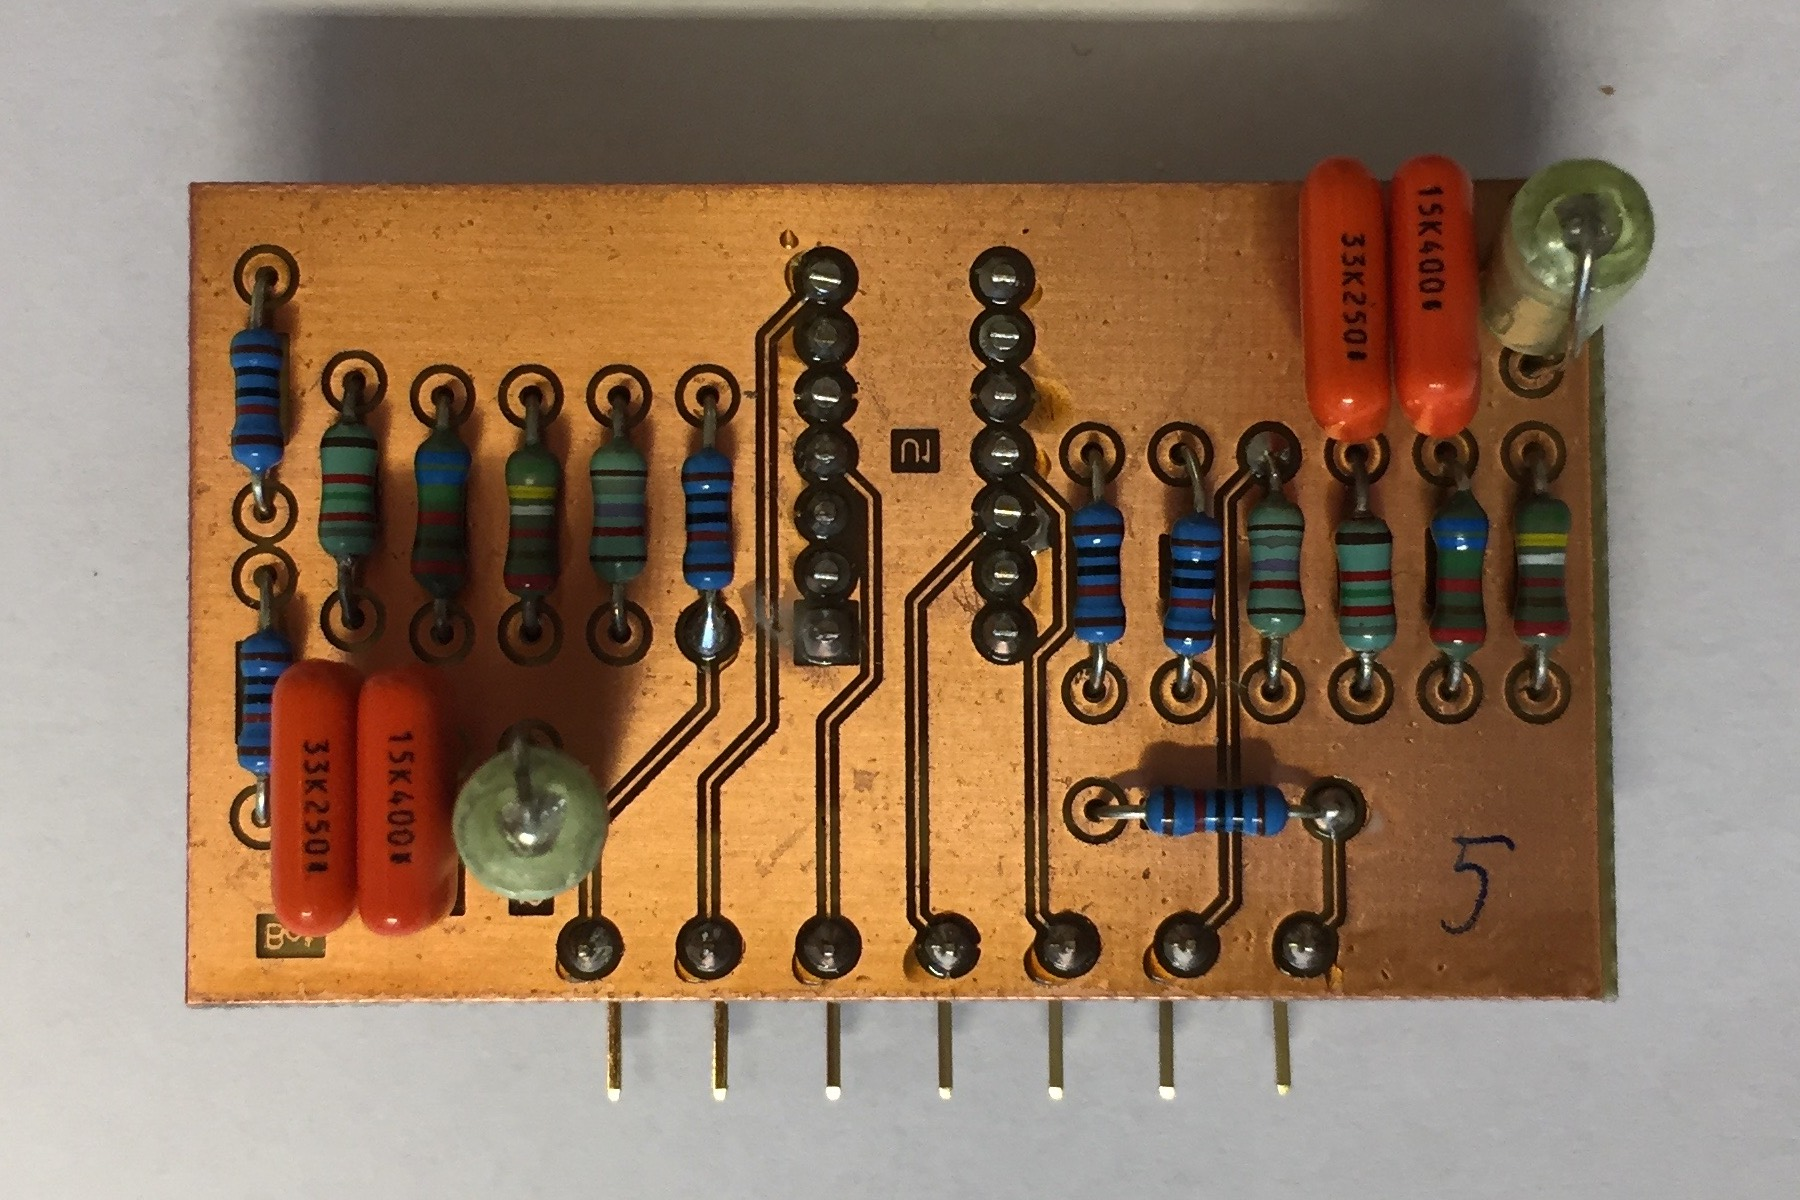
\includegraphics[resolution=300,width=\textwidth/2]{ProductShots/Filter5Front}
	\caption{Færdigt filter for $\pm$5.24dB}
	\label{fig:Filter5Front}
\end{figure}
\noindent
%
%
\begin{table}[H]
\centering
\begin{tabular}{|c|r|r|r|}
\hline
\multicolumn{1}{|l|}{Komponenter} & \multicolumn{1}{l|}{Beregnet} & \multicolumn{1}{l|}{Brugt} & \multicolumn{1}{l|}{Afvigelse [$\%$]}\\ \hline
$R_i$ & 10k$\Omega$ & 10k$\Omega$ & 0\\ \hline
$R_F$ & 33.42k$\Omega$ & 33.2k$\Omega$ & 0.6583 \\ \hline
$R_1$ & 67.502k$\Omega$ & 66.5k$\Omega$ & 1.4844 \\ \hline
$R_2$ & 45.149k$\Omega$ & 45.3k$\Omega$ & 0.3344 \\ \hline
$R_3$ & 30.198k$\Omega$ & 30.1k$\Omega$ & 0.3245 \\ \hline
$C_1$ & 28.673nF & 33nF & 15.0909 \\ \hline
$C_2$ & 16.303nF & 15nF & -7.9924 \\ \hline
$C_3$ & 9.269nF & 10nF & 7.8865 \\ \hline
\end{tabular}
\caption{Komponentværdier for de filtre der forstærker $\pm$10.48dB.}
\label{tab:TilpasningAfFiltre10.48}
\end{table}
%
\begin{figure}[H]
	\centering
	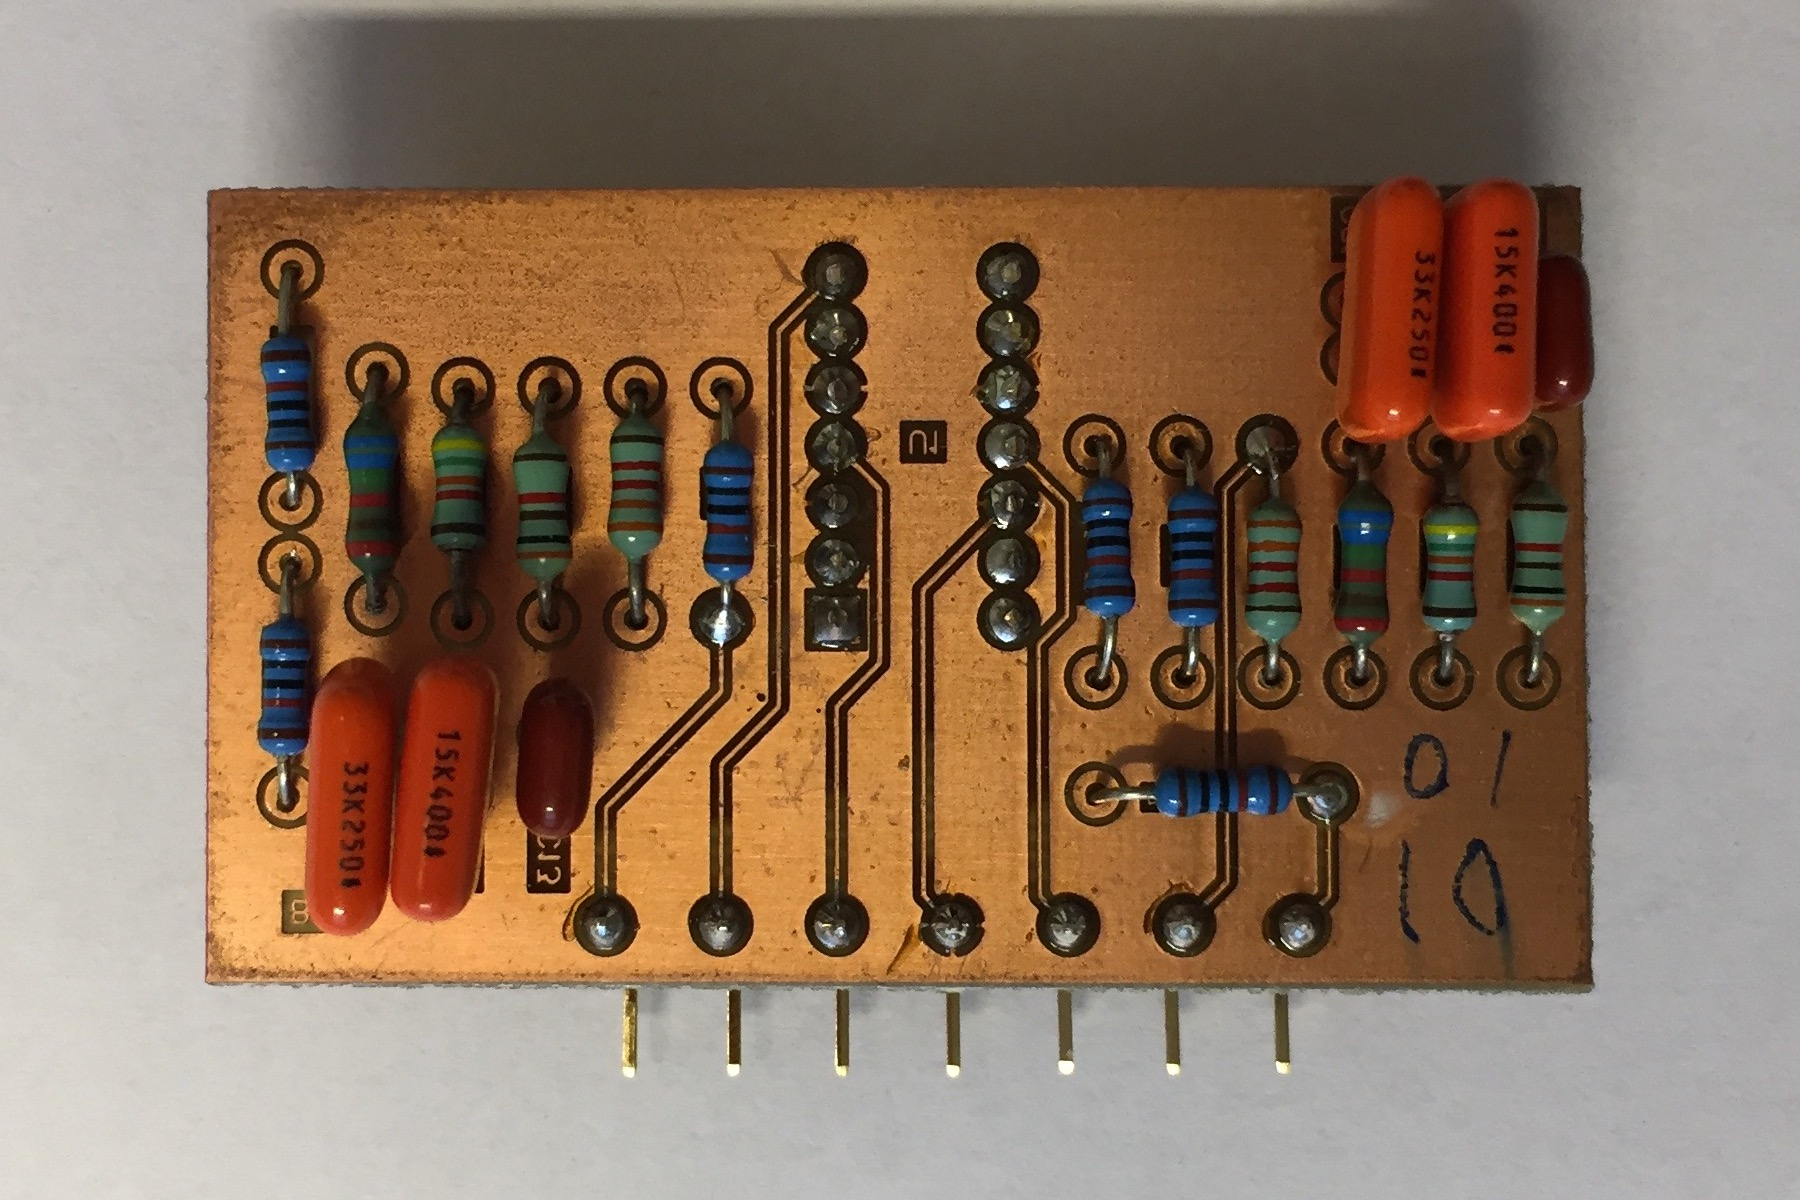
\includegraphics[resolution=300,width=\textwidth/2]{ProductShots/Filter10Front}
	\caption{Færdigt filter for $\pm$10.48dB}
	\label{fig:Filter10Front}
\end{figure}
\noindent
%
%
\begin{table}[H]
\centering
\begin{tabular}{|c|r|r|r|}
\hline
\multicolumn{1}{|l|}{Komponenter} & \multicolumn{1}{l|}{Beregnet} & \multicolumn{1}{l|}{Brugt} & \multicolumn{1}{l|}{Afvigelse [$\%$]}\\ \hline
$R_i$ & 10k$\Omega$ & 10k$\Omega$ & 0\\ \hline
$R_F$ & 111.686k$\Omega$ & 107k$\Omega$ & 4.1957 \\ \hline
$R_1$ & 90.413k$\Omega$ & 88.7k$\Omega$ & 1.8946 \\ \hline
$R_2$ & 40.448k$\Omega$ & 40.2k$\Omega$ & 0.6131 \\ \hline
$R_3$ & 18.095k$\Omega$ & 17.8k$\Omega$ & 1.6303 \\ \hline
$C_1$ & 14.318nF & 15nF & 4.7632 \\ \hline
$C_2$ & 12.172nF & 12.5nF & 2.6947 \\ \hline
$C_3$ & 10.347nF & 10nF & -3.3536 \\ \hline
\end{tabular}
\caption{Komponentværdier for de filtre der forstærker $+$20.96dB.}
\label{tab:TilpasningAfFiltre20.96}
\end{table}
%
\begin{figure}[H]
	\centering
	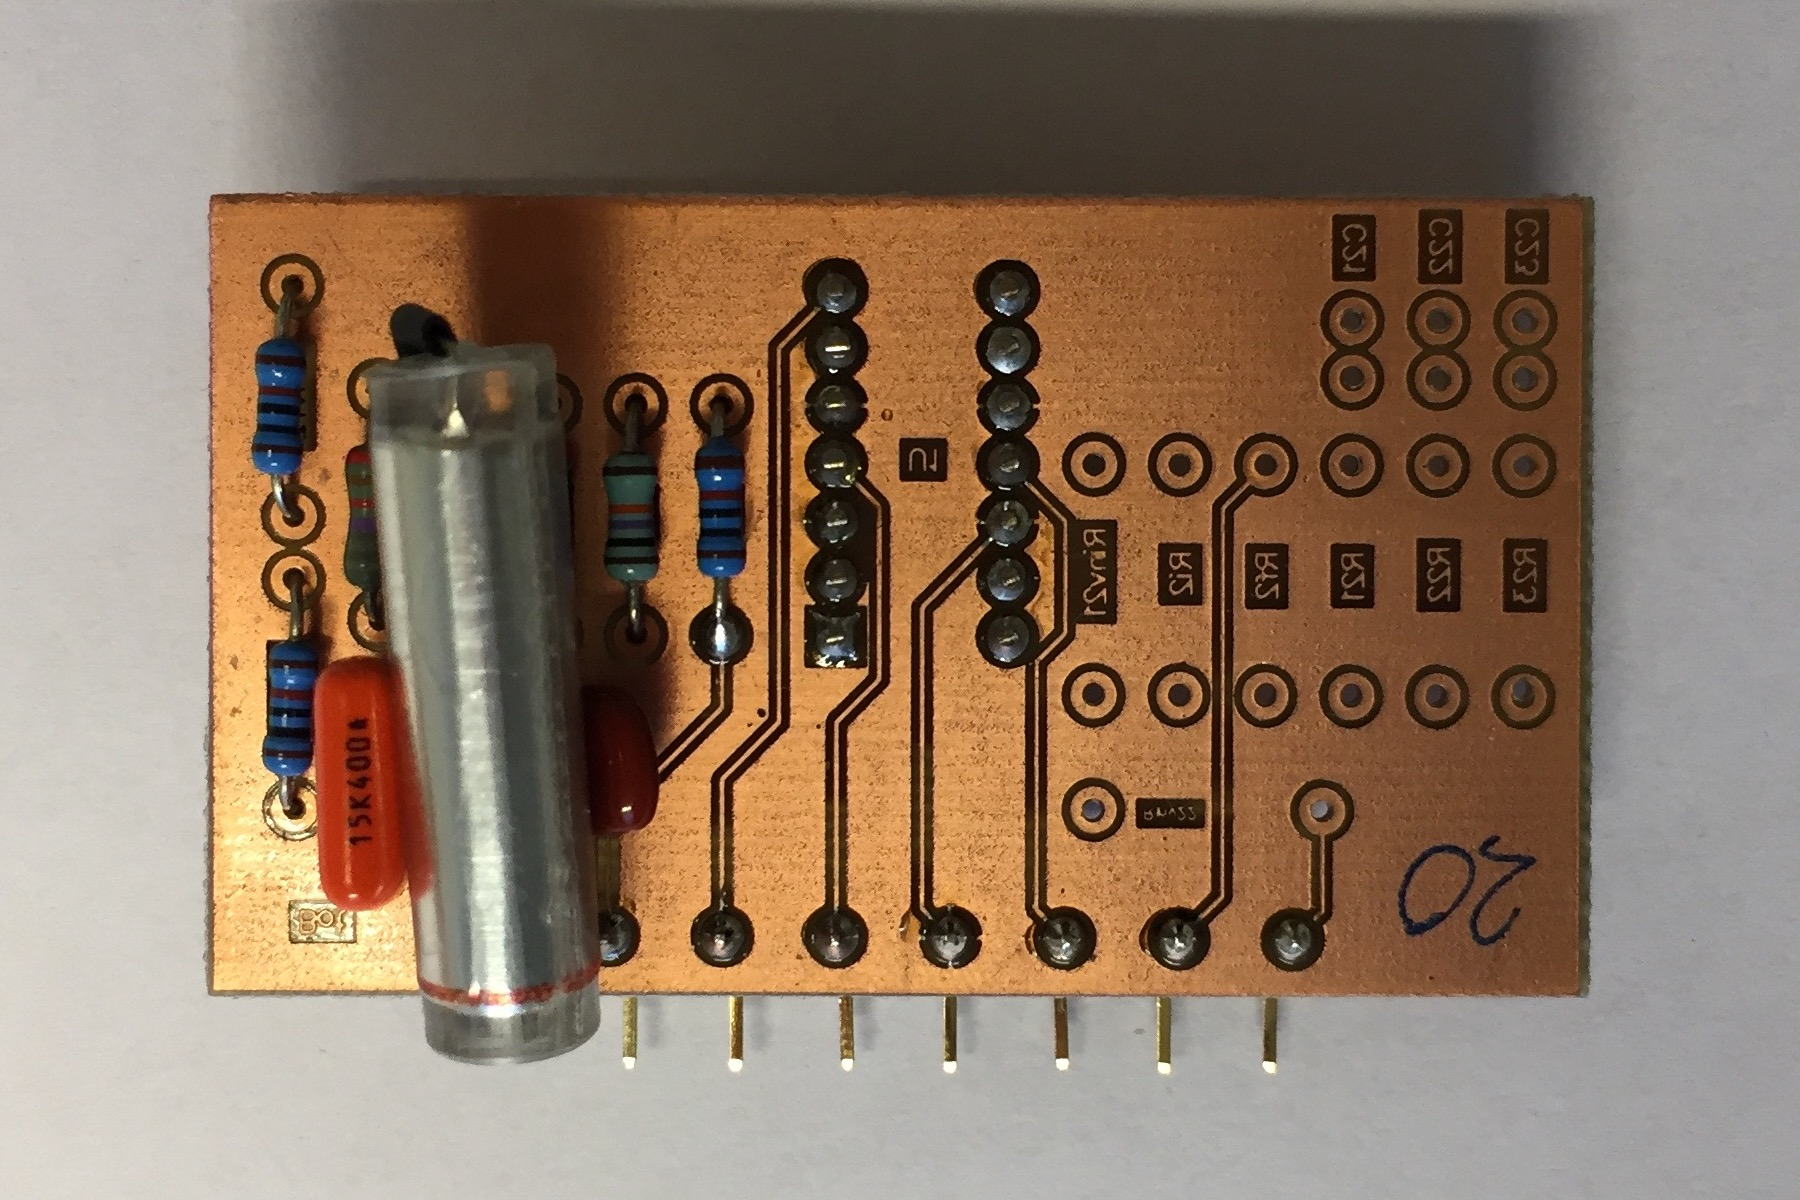
\includegraphics[resolution=300,width=\textwidth/2]{ProductShots/Filter20Front}
	\caption{Færdigt filter for $+$20.96dB}
	\label{fig:Filter20Front}
\end{figure}
%
\newpage
\noindent
%
De beregnede og brugte komponentværdier for de syv filtre, fremsat i \autoref{tab:TilpasningAfFiltre2.62}, \autoref{tab:TilpasningAfFiltre5.24}, \autoref{tab:TilpasningAfFiltre10.48} og \autoref{tab:TilpasningAfFiltre20.96}, afbilledes på \autoref{fig:UdregnetKontraPraktiskGain}.
%
\begin{figure}[H]
	\centering
	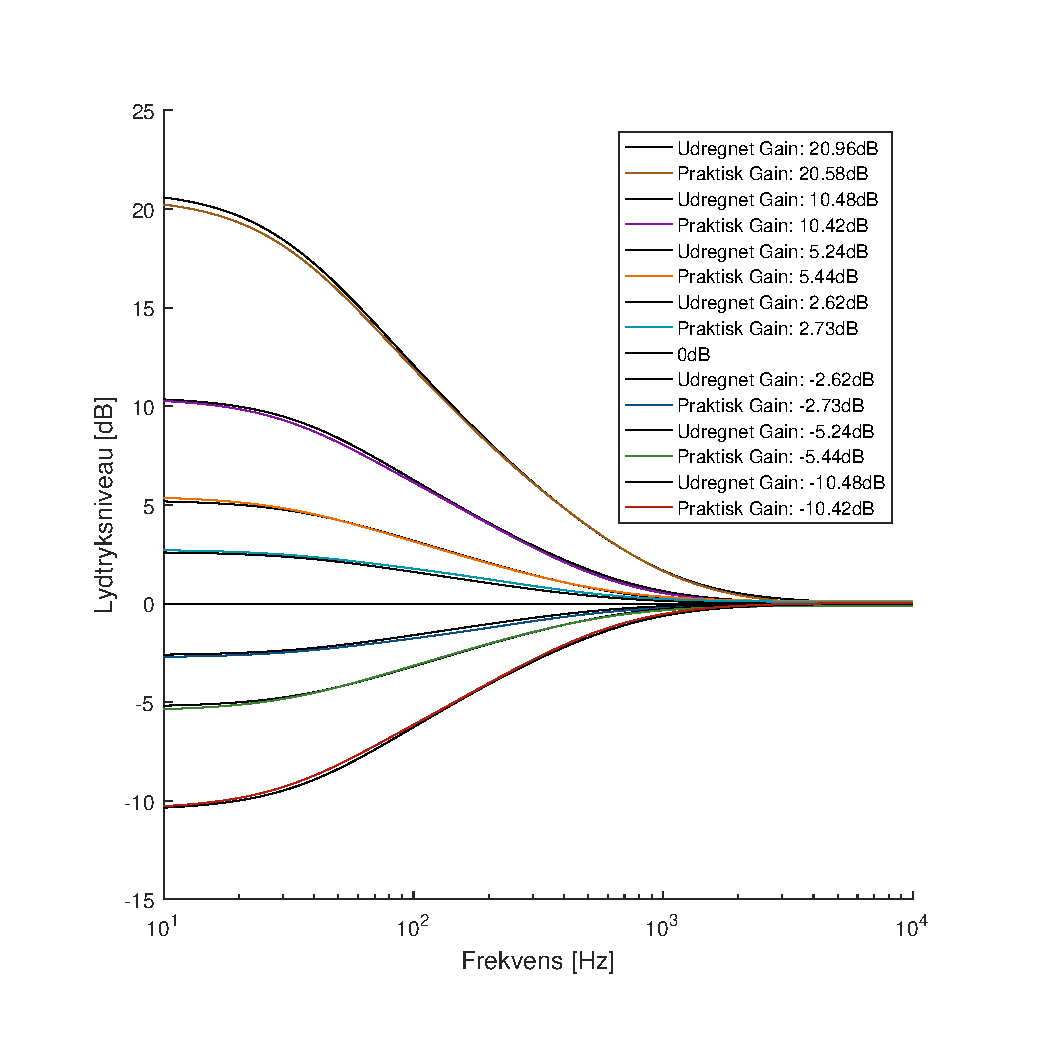
\includegraphics[resolution=300,width=\textwidth]{Figure/DesignAfFilter/UdregnetKontraPraktiskGain.pdf}
	\caption{Kurverne for de beregnede komponentværdier og de brugte komponentværdier sammenholdes. Hvor 0dB angiver én gangs forstærkning.}
	\label{fig:UdregnetKontraPraktiskGain}
\end{figure}
\noindent
%
Ud fra \autoref{fig:UdregnetKontraPraktiskGain} tyder det på, at de afvigelser der måtte være mellem de beregnede og de brugte komponentværdier er af minimal betydning. Data til \autoref{fig:UdregnetKontraPraktiskGain} forefindes i vedlagte mappe, som er navngivet: \textit{SupplerendeMateriale}. 

 
